\chapter{Background} % 2

% Questo capitolo ha l'obiettivo di presentare i principali concetti teorici e le nozioni fondamentali necessarie per comprendere gli argomenti trattati nei capitoli successivi. Saranno quindi introdotti gli aspetti essenziali su cui si fonda lo sviluppo del lavoro descritto in questa tesi.

\section{Malware e botnet} % 2.1

In generale, qualsiasi software progettato per compromettere la riservatezza, l'integrità o la disponibilità di un sistema informatico, di una rete o dei dati di un utente può essere classificato come \emph{malware} \cite{sikorski2012malware}, abbreviazione di \emph{malicious software}. Il malware può assumere diverse forme e, in base al proprio obiettivo, può appartenere a una o più categorie, tra cui, ad esempio, \emph{backdoor}, \emph{information stealer}, \emph{launcher}, \emph{worm}, \emph{virus} e altre. % Capitolo 0

% Il malware può essere sviluppato con differenti finalità: il furto di informazioni, il danneggiamento dei sistemi o l'accesso a dispositivi non autorizzato.
% Forme del malware: programmi eseguibili, \textit{script} o codice incorporato in altri software
% Altre categorie: dropper, downloader

Nel corso degli anni, l'evoluzione delle infrastrutture di rete e il cambiamento delle abitudini tecnologiche hanno portato a un aumento del numero di dispositivi connessi e del tempo durante il quale essi rimangono online. Questo fenomeno, unito alla presenza di vulnerabilità di sicurezza nei sistemi, ha favorito lo sviluppo e la diffusione di nuove minacce informatiche, tra cui le botnet, oggi considerate una delle principali minacce nel panorama della sicurezza informatica.

Una \emph{botnet} \cite{silva2013botnets} è una rete di host compromessi, detti \emph{bot}, controllati da remoto da uno o più attaccanti, chiamati \emph{botmaster}. Il malware installato sul dispositivo consente al botmaster di controllare da remoto i dispositivi e di eseguire azioni malevole. % Capitolo 1-2

Dal punto di vista degli attaccanti, le botnet rappresentano uno strumento estremamente redditizio, poiché consentono di ottenere un ritorno economico attraverso lo sfruttamento dei dispositivi compromessi. Una volta infettati, tali dispositivi possono essere impiegati simultaneamente per eseguire attività malevole su larga scala, generando danni economici per utenti, aziende e Internet Service Provider (ISP). Le botnet possono fungere da infrastruttura per numerose attività criminali online, tra cui invio di spam, distribuzione di malware, furto di informazioni e attacchi \emph{Distributed Denial of Service} (DDoS). Tra queste, gli attacchi DDoS rappresentano uno degli utilizzi più diffusi, poiché consentono di sfruttare la capacità trasmissiva complessiva dei dispositivi compromessi per sovraccaricare il bersaglio e rendere i suoi servizi indisponibili. % frodi informatiche,

\subsection{Architettura} % 2.1.1

Il componente fondamentale di una botnet è l'infrastruttura di \emph{Command-and-Control} (C\&C) \cite{silva2013botnets}, che permette la comunicazione tra il botmaster e i bot compromessi, coordinandone le attività. Attraverso il canale C\&C vengono trasmessi i comandi, che i bot interpretano ed eseguono sul dispositivo infetto. % Capitolo 2.3

Per realizzare tale comunicazione possono essere impiegati diversi protocolli di rete, che, così come le funzionalità implementate, variano in funzione degli obiettivi della botnet. Oltre alla trasmissione dei comandi, il canale C\&C consente di mantenere il controllo dei bot, distribuire aggiornamenti del malware e raccogliere informazioni dai dispositivi compromessi. 

% Per realizzare tale comunicazione possono essere impiegati diversi protocolli di rete. I protocolli utilizzati, così come le funzionalità implementate, variano in funzione degli obiettivi della botnet. 

L'architettura dell'infrastruttura C\&C influenza direttamente la robustezza e la capacità di sopravvivenza della botnet. Le architetture possono essere ricondotte principalmente a tre modelli: centralizzato, distribuito e ibrido \cite{silva2013botnets, hachem2011topology}. % Capitolo 2.6, Pagina 3

Nel \emph{centralized C\&C model}, il botmaster individua uno o più host che fungono da server C\&C e costituiscono il punto di contatto per i bot compromessi, secondo tre principali configurazioni topologiche. La topologia a \emph{stella singola} prevede un unico server C\&C al quale si collegano tutti i bot, secondo un'organizzazione analoga al modello \emph{client-server} (\Cref{fig:botnet_topology} (a)). La topologia a \emph{stella multi-server} utilizza invece più server C\&C, tra loro interconnessi e tra i quali vengono distribuiti i bot, aumentando ridondanza e scalabilità dell'infrastruttura (\Cref{fig:botnet_topology} (b)). Infine, la topologia \emph{gerarchica} prevede che alcuni bot assumano la funzione di \emph{proxy server}, fungendo da intermediari tra gli altri bot e i server C\&C, riducendo il numero di bot che conosce direttamente l'indirizzo del server C\&C (\Cref{fig:botnet_topology} (c)).

% Il C\&C server può essere una macchina compromessa o un provider legittimo. Ovviamente i protocolli sui canali di comunicazioni sono protetti per evitare l'eavesdropping. Il modello centralizzato è quello più utilizzato grazie alla sua semplicità di implementazione e ridotta latenza, con gli svantaggi di facilità di detection e compromissione.

Il \emph{distributed C\&C model} adotta invece un'architettura decentralizzata, tipicamente basata su reti \emph{peer-to-peer} (P2P), dove non esiste un server C\&C centrale, i bot comunicano tra loro e il botmaster impartisce i comandi collegandosi a un nodo qualsiasi della rete (\Cref{fig:botnet_topology} (d)). Sebbene questo modello sia generalmente più complesso da realizzare, l'infrastruttura è più resistente alle attività di rilevamento e smantellamento. Infine, l'\emph{hybrid C\&C model} combina, secondo diversi approcci, elementi dei modelli centralizzato e distribuito, spesso assegnando ruoli differenti ai nodi. % l'assenza di un punto centrale di controllo elimina un singolo punto di fallimento. 

% Le principali topologie associate ai modelli centralizzato e distribuito sono illustrate nella \Cref{fig:botnet_topology}.

\begin{figure}[t]
    \centering
    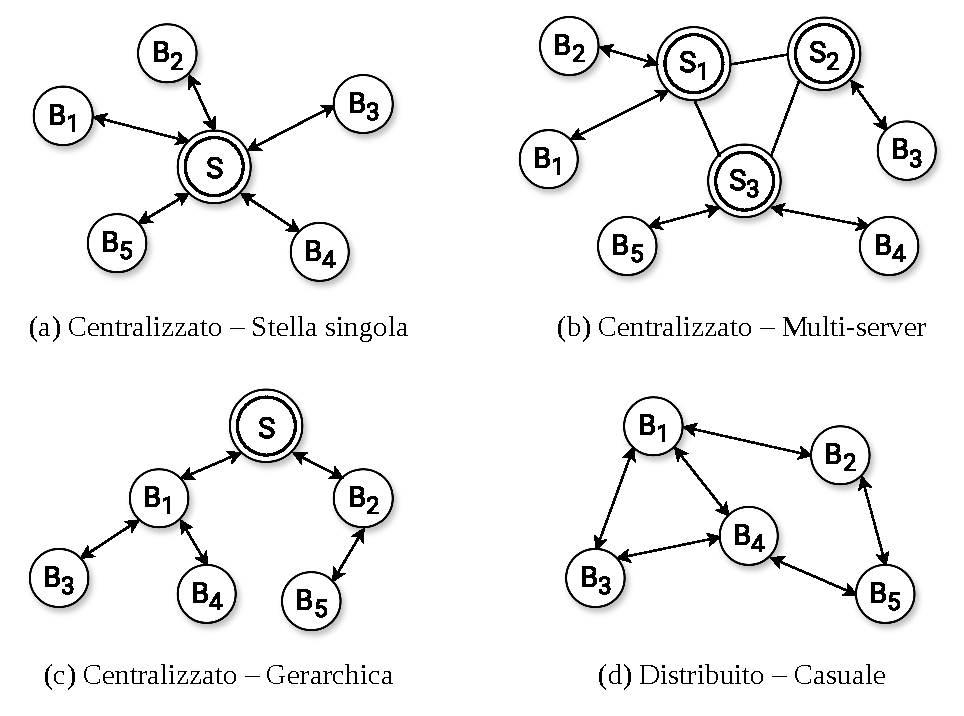
\includegraphics[width=0.75\textwidth]{img/botnet_topology.pdf}
    \caption[Topologie delle botnet]{
        Modelli e topologie delle botnet. Adattata da \cite{hachem2011topology}.
    }
    \label{fig:botnet_topology}
\end{figure}

\subsection{Ciclo di vita} % 2.1.2

Secondo il modello proposto in \cite{silva2013botnets} e rappresentato in \Cref{fig:botnet_lifecycle}, il ciclo di vita di una botnet può essere generalmente suddiviso in cinque fasi, realizzate secondo modalità differenti in funzione dell'architettura C\&C adottata:

% Il ciclo di vita di una botnet può essere generalmente suddiviso in cinque fasi, la cui implementazione può variare in funzione dell'architettura C\&C adottata, secondo il modello proposto in \cite{silva2013botnets}: % Capitolo 2.4

% \begin{enumerate}[label=Fase (\arabic*)., leftmargin=*] \end{enumerate}

\begin{description}
    \item[Infezione iniziale.] Un host viene compromesso attraverso dei vettori di attacco comuni e diventa un potenziale bot.
    \item[Iniezione secondaria.] Il malware iniziale, che può essere un \emph{dropper} o un \emph{downloader}, scarica o attiva il componente principale della botnet, trasformando il dispositivo in un bot controllabile dal botmaster.
    \item[Connessione C\&C.] Il nuovo bot stabilisce una connessione con l'infrastruttura C\&C per registrare la propria presenza e per mettersi in attesa di istruzioni. L'individuazione dei nodi o degli \emph{endpoint} dell'infrastruttura C\&C può avvenire tramite metodi statici (indirizzi IP o nomi di dominio \emph{hardcoded}) oppure con tecniche più sofisticate, come i \emph{Domain Generation Algorithm} (DGA).
    %\item[Connessione C\&C.] Il nuovo bot deve stabilire una connessione con l'infrastruttura C\&C per registrare la propria presenza e per mettersi in attesa di istruzioni o aggiornamenti. La risoluzione dell'indirizzo del server C\&C avviene tramite metodi statici (indirizzi IP o nomi di dominio \emph{hardcoded}) oppure mediante tecniche più sofisticate, come i \emph{Domain Generation Algorithm} (DGA). % hardcoded nel binario
    \item[Attività malevole.] Il bot è ora nella fase operativa, è pronto per ricevere i \emph{payload} di comando ed eseguire le attività malevole ordinate dal botmaster.
    \item[Manutenzione e aggiornamento.] Alla fine la botnet entra nella fase di manutenzione, che ha l'obiettivo di garantire la sua sopravvivenza nel lungo periodo. Il botmaster può inviare aggiornamenti del malware, con lo scopo di correggere vulnerabilità o aggiungere nuove funzionalità.
\end{description}

Il modello C\&C, in particolare nelle architetture centralizzate, introduce però una vulnerabilità intrinseca \cite{silva2013botnets}: la necessità per i bot di comunicare con l'infrastruttura di comando espone l'attività malevola all'osservazione, costituendo un punto debole sfruttato dalle metodologie di rilevamento. Il traffico analizzato include l'\textit{handshake} iniziale, con lo scambio di identificativi e l'eventuale \emph{profiling} dell'host compromesso, il \emph{beaconing} periodico verso un \emph{C\&C endpoint} per segnalare la disponibilità del bot (\emph{keepalive}) e i payload di comando. % Capitolo 2.4

\begin{figure}[t]
    \centering
    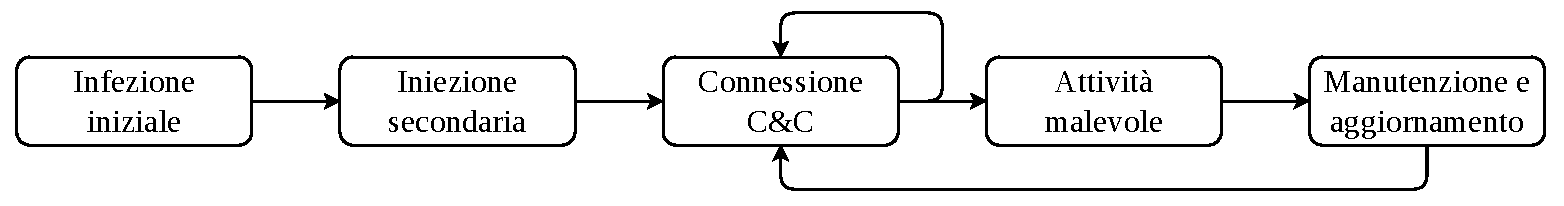
\includegraphics[width=0.95\textwidth]{img/botnet_lifecycle.pdf}
    \caption[Ciclo di vita di una botnet]{
        Ciclo di vita di una botnet. Adattata da \cite{silva2013botnets}.
    }
    \label{fig:botnet_lifecycle}
\end{figure}

\subsection{IoT botnet e Mirai} \label{sec:mirai} % 2.1.3

% Le botnet costituiscono una minaccia informatica presente da diversi anni. Nell'ambito della cosiddetta Quarta Rivoluzione Industriale. La compromissione di tali dispositivi può quindi avere implicazioni sia per la sicurezza dei sistemi sia per la privacy degli utenti.

% Parallelamente alla crescita delle botnet, si sono evolute anche le tecniche di difesa, che possono essere di tipo reattivo, intervenendo dopo la compromissione, oppure preventivo, con l'obiettivo di impedire o limitare l'infezione prima che questa si verifichi. Nonostante il progressivo rafforzamento dei meccanismi di protezione, la continua evoluzione delle tecnologie e dei dispositivi connessi ha offerto nuove opportunità agli attaccanti, contribuendo all'espansione della superficie d'attacco. In particolare, la rapida diffusione dei dispositivi appartenenti all'\textit{Internet of Things} (IoT) ha favorito la creazione e la diffusione di botnet su larga scala, a causa delle risorse hardware limitate e di configurazioni di sicurezza spesso inadeguate.

La progressiva diffusione delle tecnologie e dei dispositivi appartenenti all'\emph{Internet of Things} (IoT) ha contribuito ad ampliare la superficie di attacco e, di conseguenza, le opportunità per la proliferazione delle botnet \cite{lefoane2025iot}. L'adozione dell'IoT ha infatti interessato un numero crescente di settori, dalle applicazioni domestiche a quelle industriali, e i dispositivi IoT possono raccogliere, elaborare e trasmettere attraverso Internet grandi quantità di dati, spesso di grande valore e caratterizzati da requisiti di sicurezza e riservatezza particolarmente stringenti.

% L'adozione dell'IoT ha infatti interessato un numero crescente di settori, dalle applicazioni domestiche, come le smart home, a quelle sanitarie, energetiche e industriali. I dispositivi IoT sono interconnessi e possono raccogliere, elaborare e trasmettere attraverso Internet grandi quantità di dati, spesso caratterizzati da requisiti di sicurezza e riservatezza particolarmente elevati.

Le caratteristiche dell'ecosistema IoT rappresentano uno dei principali fattori che può rendere questi dispositivi vulnerabili alla compromissione da parte degli attaccanti \cite{lefoane2025iot}. Molti di essi presentano risorse computazionali e capacità di memoria limitate, rendendo più complessa l'adozione di meccanismi di sicurezza avanzati senza incidere sulle loro funzionalità e prestazioni. A ciò si aggiungono configurazioni di sicurezza talvolta insufficienti, che possono trasformare i dispositivi in punti deboli dell'ecosistema, facilitandone l'arruolamento all'interno di una botnet.

% , ma anche campagne di \emph{phishing} e attacchi \emph{ransomware}

Questi elementi hanno favorito la diffusione delle \emph{IoT botnet} e degli attacchi condotti con esse, principalmente di tipo DDoS. Le IoT botnet rappresentano una sfida rilevante per la sicurezza informatica anche dal punto di vista del rilevamento, poiché, a differenza di alcuni attacchi condotti attraverso botnet tradizionali, possono generare traffico proveniente da indirizzi di rete legittimi e con caratteristiche difficili da distinguere dal traffico normale.

L'impatto potenziale delle IoT botnet è stato evidenziato in modo significativo dalla diffusione a partire dall'agosto 2016 della botnet \emph{Mirai}. In pochi mesi, Mirai ha raggiunto centinaia di migliaia di dispositivi compromessi ed è stata impiegata per alcuni dei più grandi attacchi DDoS osservati fino ad allora, colpendo servizi e organizzazioni di rilievo in Europa e negli Stati Uniti \cite{lefoane2025iot, antonakakis2017mirai}. La minaccia rappresentata dalle botnet, in particolare nell'ambito IoT, rimane tuttavia attuale \cite{nokia2025ddos}: nel 2025 sono state osservate nuove generazioni di varianti della famiglia Mirai, con oltre trentamila dispositivi IoT compromessi e una capacità di attacco stimata fino a $30 \; Tbps$. % Trend 4

\emph{Mirai} \cite{antonakakis2017mirai} è una famiglia di malware di tipo \emph{worm-like} e rappresenta un'evoluzione della preesistente botnet \emph{BASHLITE}, conosciuta anche come \emph{Gafgyt}, che infettava dispositivi Linux attraverso il \emph{brute force} di credenziali predefinite. La sua rapida espansione è stata favorita dalla semplicità del malware, dall'efficienza della scansione della rete e, soprattutto, dallo sfruttamento di credenziali predefinite deboli o mai modificate sui dispositivi IoT. La sua architettura è centralizzata e prevede tre componenti principali, il C\&C, il \emph{report server} e il \emph{loader}, che costituiscono l'infrastruttura interposta tra i bot e il botmaster, mentre il suo flusso operativo è illustrato nella \Cref{fig:mirai_operation}.

% , permettendole di compromettere dispositivi eterogenei su larga scala.

La propagazione di Mirai avviene attraverso un rapido meccanismo di scanning che invia in modo asincrono e \emph{stateless} pacchetti TCP SYN verso indirizzi IPv4 pseudocasuali, sulle porte $23$ e $2323$, utilizzate dal protocollo Telnet. Quando viene identificata una potenziale vittima, Mirai tenta di stabilire una connessione mediante un attacco di tipo brute force, provando diverse coppie di username e password selezionate da un pool di 62 credenziali. Rispetto a BASHLITE, il set di credenziali viene ampliato con combinazioni specifiche per router consumer e dispositivi IoT.

Una volta completato con successo il login, Mirai invia al report server l'indirizzo IP della vittima e le relative credenziali. Questo evento attiva il loader, che procede all'infezione del dispositivo vulnerabile eseguendo il login, identificando l'architettura e l'ambiente di esecuzione e scaricando il binario specifico per il sistema. Al termine dell'infezione, il binario scaricato viene eliminato e il malware procede all'offuscamento del nome del processo e all'interruzione dei processi associati a esecuzioni o infezioni concorrenti, comprese altre varianti di Mirai. A questo punto, il bot effettua la scansione di nuove potenziali vittime e, simultaneamente, rimane in ascolto dei comandi provenienti dal C\&C, che possono essere utilizzati per condurre attacchi DDoS. % senza implementare meccanismi di persistenza. i processi concorrenti utilizzano le porte 22 e 23

\begin{figure}[t]
    \centering
    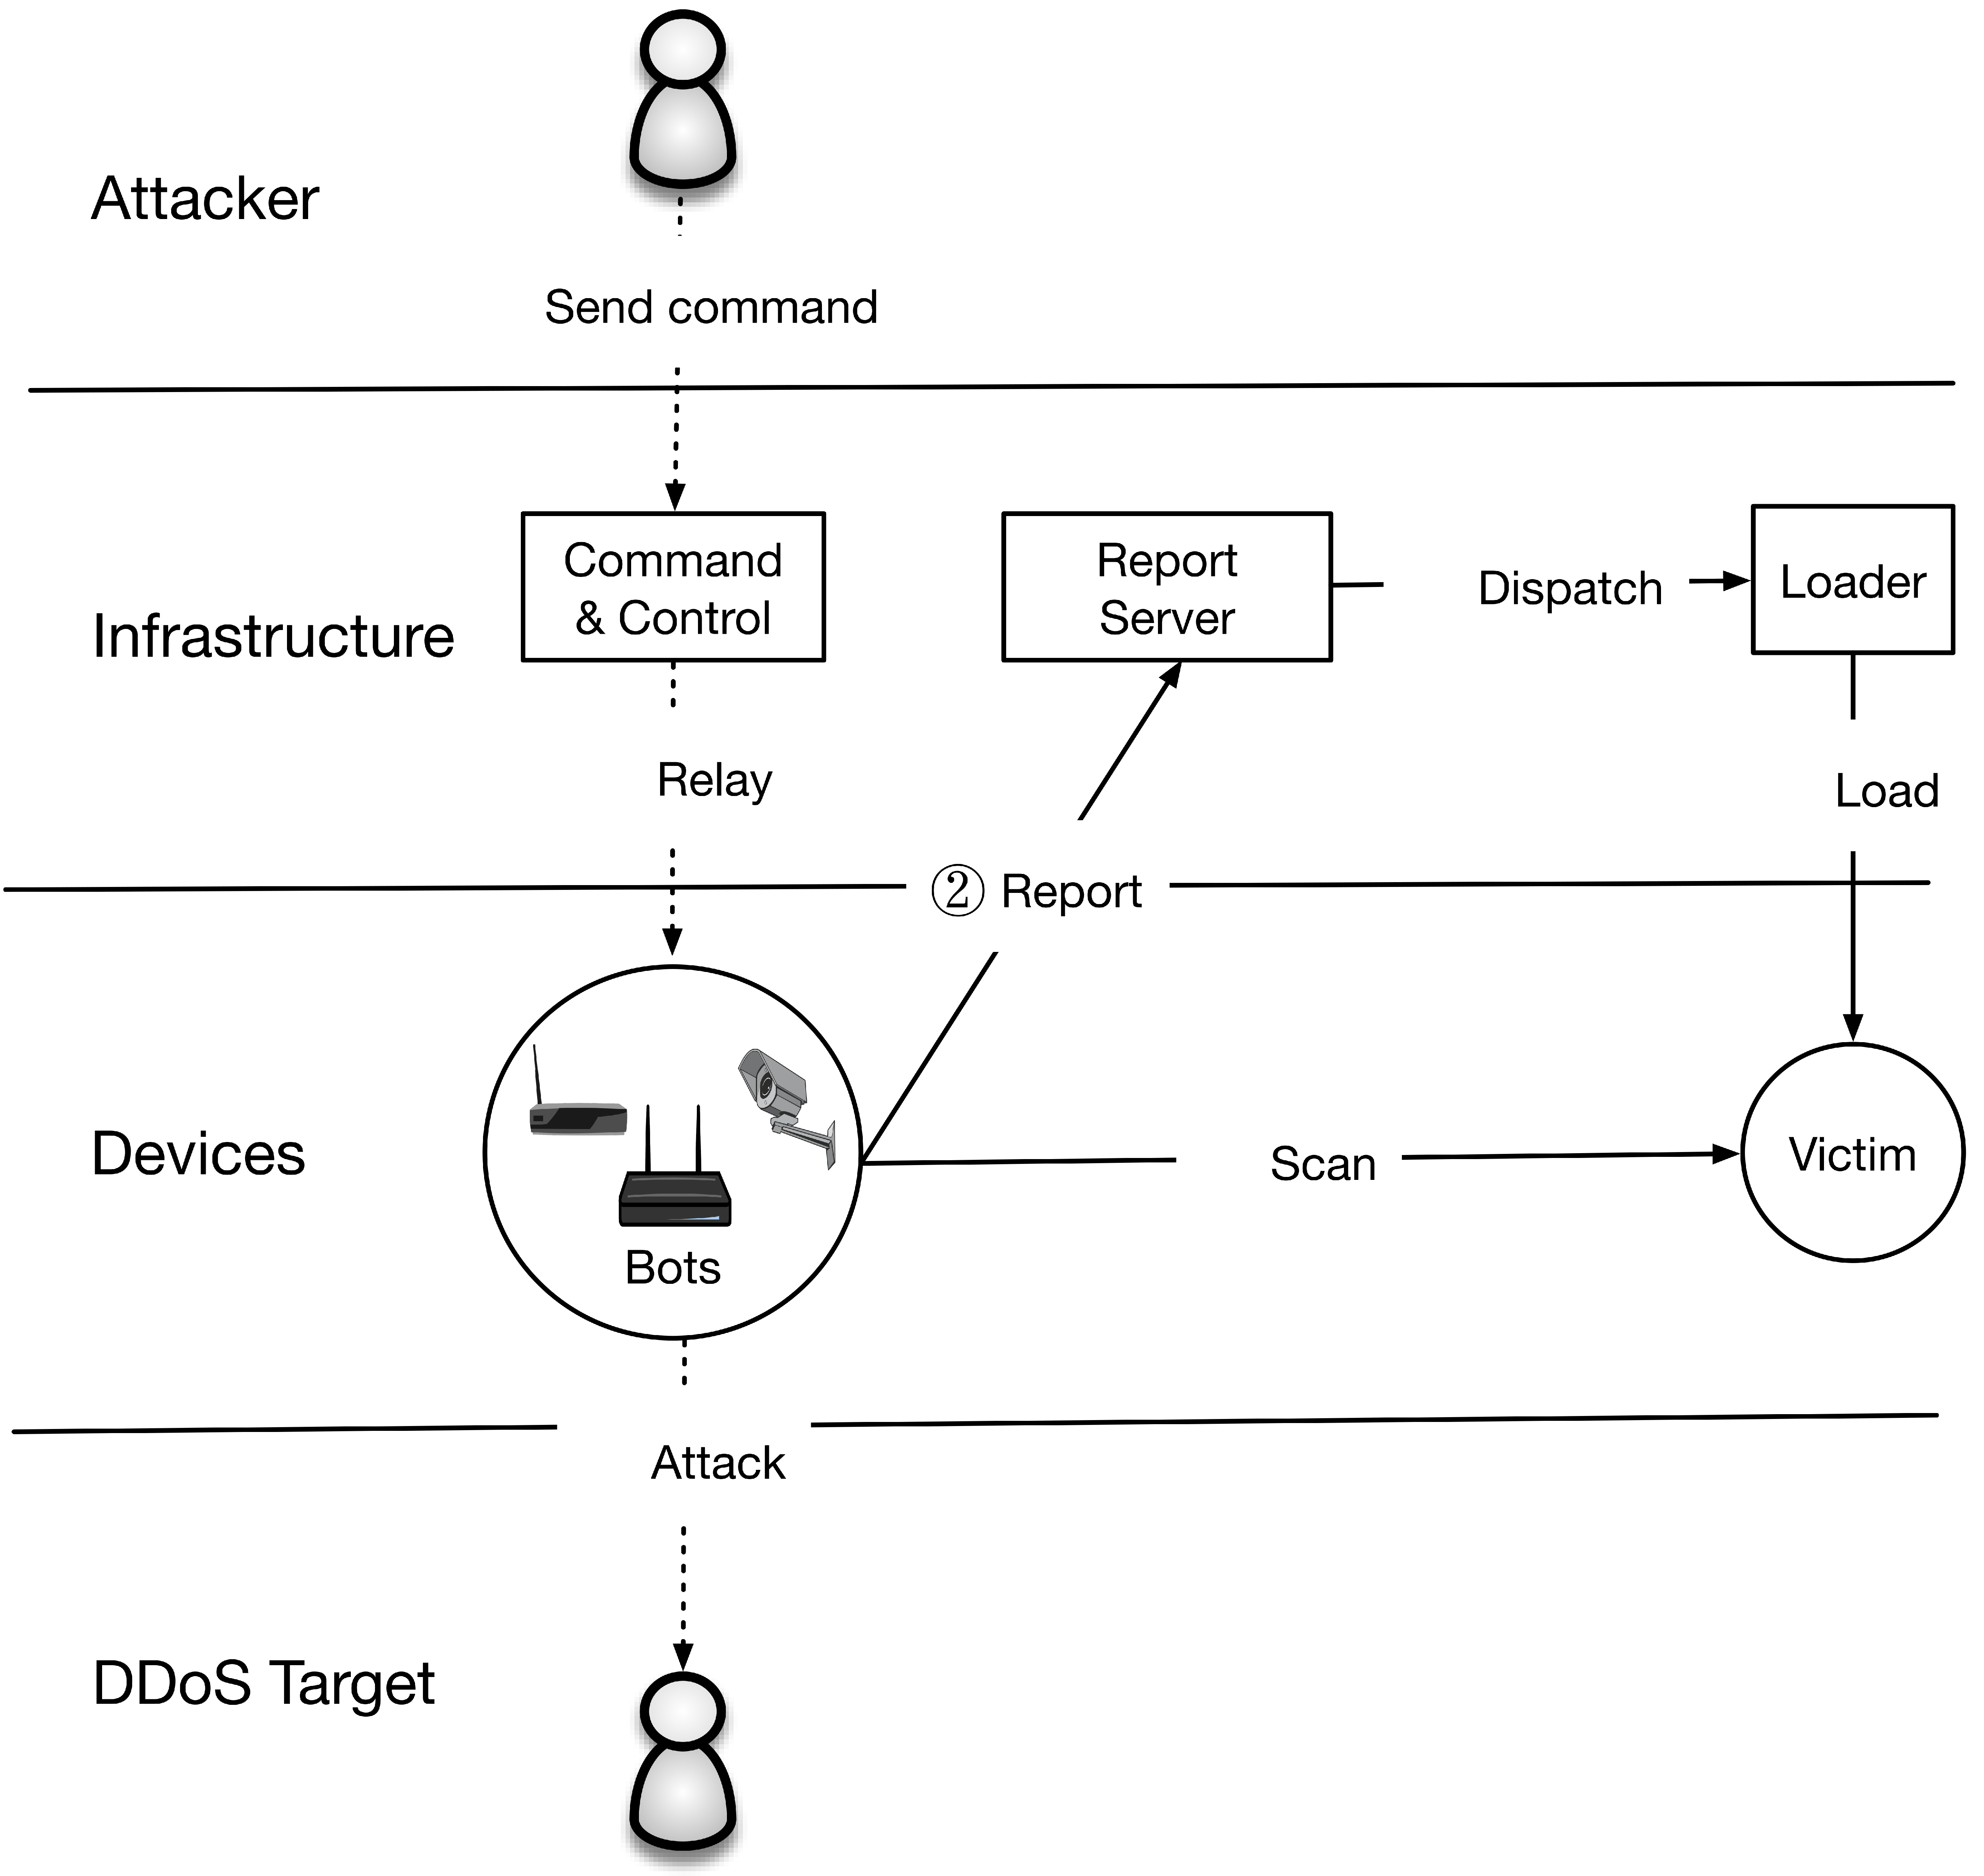
\includegraphics[width=0.65\textwidth]{img/mirai_operation.pdf}
    \caption[Schema di funzionamento della botnet Mirai]{
        Schema di funzionamento della botnet Mirai. Adattata da \cite{antonakakis2017mirai}.
    }
    \label{fig:mirai_operation}
\end{figure}

Un evento significativo nella storia di Mirai è stato il rilascio pubblico del codice sorgente nell'ottobre 2016 \cite{antonakakis2017mirai}, che ha favorito la proliferazione di nuove varianti e la rapida introduzione di nuove funzionalità. Queste spaziano dal miglioramento delle capacità di infezione, attraverso l'ampliamento delle credenziali utilizzate e il potenziamento dei meccanismi di protezione dalle infezioni concorrenti, fino all'impiego di binari progettati per complicare l'attività di SRE, ad esempio mediante tecniche di packing.

Sebbene Mirai continui a essere utilizzata, oggi il principale rischio, come già osservato in precedenza, è rappresentato dalle sue varianti emergenti. Queste possono derivare sia da famiglie di malware preesistenti, come Gafgyt, che hanno incorporato moduli o caratteristiche di Mirai, sia dallo sviluppo di nuove famiglie basate sul codice sorgente. Tra le varianti successive più rilevanti si annoverano \cite{hojun2024variant}:

\begin{description}
    \item[\textbf{Hajime} \normalfont(2016).] Utilizza una blacklist per escludere determinati indirizzi IP dagli attacchi, supporta l'aggiornamento di funzionalità e adotta una comunicazione peer-to-peer, basata su BitTorrent.
    \item[\textbf{Satori} \normalfont(2017).] Per la sua diffusione sfrutta vulnerabilità del protocollo \emph{Universal Plug and Play} (UPnP) presenti in router Huawei e dispositivi basati sul Realtek SDK, senza ricorrere allo scanning. Da Satori è derivata a sua volta \emph{Coin Robber}, che sfrutta vulnerabilità di Claymore Miner per il furto di criptovalute.
    \item[\textbf{IoT Reaper} \normalfont(2018).] Sfrutta vulnerabilità note nei servizi HTTP di dispositivi IoT e, a differenza della connessione persistente di Mirai con il C\&C, effettua periodicamente richieste HTTP non cifrate. % utilizza il linguaggio Lua
    \item[\textbf{Mozi} \normalfont(2019).] Combina caratteristiche di Gafgyt, Mirai e IoT Reaper, adottando un'architettura peer-to-peer, gestita con un protocollo basato su Distributed Hash Table (DHT), che viene utilizzato per la comunicazione tra i nodi e per veicolare payload malevoli, rendendo più difficile il loro rilevamento.
    % \item Pink (2021): è stata riconosciuta come la prima botnet IoT che presenta una topologia ibrida, combinando un server C\&C centralizzato con un'architettura di rete decentralizzata. I principali bersagli sono i router con fibra ottica e oltre che per gli attacchi DDoS è stata protagonista di attacchi di inserimento di annunci all'interno di siti web HTTP. (non è variante Mirai).
\end{description}

\section{Malware analysis} % 2.2

La \textit{malware analysis} \cite{sikorski2012malware} è la disciplina che si occupa di analizzare i malware al fine di identificarne le funzionalità, comprenderne il comportamento e sviluppare adeguate contromisure per il rilevamento e la mitigazione delle minacce a essi legate. % Capitolo 0

Nel contesto della risposta a un incidente di sicurezza, la malware analysis consente di raccogliere le informazioni necessarie per ricostruire quanto accaduto, determinando gli obiettivi, le capacità e il comportamento del malware. Quando l'analista ha a disposizione un campione del malware, generalmente si tratta del file eseguibile, mentre non ha accesso al relativo codice sorgente. La comprensione del suo funzionamento richiede l'impiego di tecniche di \emph{Software Reverse Engineering} (SRE), che consentono di ricostruire la logica del programma a partire dal codice compilato. Le tecniche di SRE si dividono principalmente in due categorie, analisi statica e analisi dinamica, basate su approcci complementari.

% Tra i risultati dell'analisi vi è anche l'individuazione di elementi utili al rilevamento, tra cui le \textit{signatures} e gli \textit{Indicators of Compromise} (IoC). Questi ultimi possono essere di tipo \textit{host-based}, quando riguardano artefatti presenti sul sistema compromesso, come file creati o modificati e variazioni al registro di sistema, oppure \textit{network-based}, quando sono ricavati dall'analisi del traffico di rete e consentono di individuare comunicazioni riconducibili all'attività del malware.

% Software Reverse Engineering (SRE) involves analyzing software to uncover its design and functionality. Applications range from malware analysis to vulnerability discovery and piracy prevention. The primary goal is to reconstruct program logic and identify conditions that trigger specific code behaviors, often linked to bugs or malicious actions.

\subsection{Analisi statica} % 2.2.1

La \textit{static analysis} \cite{sikorski2012malware} consiste nell'esaminare un malware senza eseguirlo, analizzandone la struttura e il contenuto al fine di ricavarne informazioni sul funzionamento. % Capitolo 1

Le tecniche di analisi statica di base comprendono l'utilizzo di strumenti antivirus per una prima classificazione del campione, il calcolo di hash per identificarne univocamente il file e l'ispezione delle informazioni contenute nell'eseguibile, quali stringhe, intestazioni del formato binario, librerie importate o esportate. Sebbene queste tecniche consentano di ottenere rapidamente informazioni preliminari, da sole raramente permettono di comprendere completamente il comportamento del malware.

% e altri metadati utili

\subsubsection{Analisi statica del codice}

L'analisi statica avanzata si basa sull'ispezione delle istruzioni contenute nel file eseguibile del malware. Poiché tali istruzioni sono espresse in linguaggio macchina e non sono direttamente leggibili dal reverse engineer, viene utilizzato un \emph{disassembler} \cite{sikorski2012malware}, uno strumento che traduce il codice macchina nel corrispondente linguaggio assembly. Quest'ultimo fornisce una rappresentazione testuale delle istruzioni della CPU, permettendo di analizzare le operazioni eseguite dal programma a basso livello.  % Capitolo 2

Un ulteriore strumento utilizzato nell'analisi dei binari è il \emph{decompiler} \cite{sikorski2012malware}, che tenta di tradurre il codice macchina in una rappresentazione equivalente in un linguaggio di alto livello. Sebbene il risultato non corrisponda necessariamente al codice sorgente originale, questa rappresentazione introduce un maggiore livello di astrazione e può facilitare la comprensione della logica del programma.

Due dei più noti strumenti di SRE sono IDA Pro e Ghidra \cite{sikorski2012malware}. Questi software offrono un ambiente completo per l'analisi dei binari, affiancando al disassembler funzionalità di decompilazione, debugging e strumenti di supporto come la navigazione del codice, l'analisi delle funzioni e la ricostruzione dei tipi. Tuttavia, le esigenze degli sviluppatori e dei reverse engineer possono richiedere l'introduzione di funzionalità aggiuntive non direttamente disponibili. Per questo motivo Ghidra, così come altri strumenti di SRE, mette a disposizione meccanismi di scripting basati sull'\textit{Application Programming Interface} (API) della piattaforma, che consente di interagire con le funzionalità interne del software \cite{nance2026ghidrabook}. Attraverso tale API è possibile creare ed eseguire script in Java e Python per automatizzare operazioni, sviluppare strumenti di analisi ed estendere le funzionalità della piattaforma mediante plugin dedicati. % Capitolo 14

% Attraverso tale API è possibile creare ed eseguire script in Java e Python che possono variare da semplici automazioni di operazioni comuni fino alla realizzazione di strumenti più complessi per l'analisi dei programmi, arrivando anche a estendere le capacità della piattaforma mediante plugin dedicati.

\subsubsection{Limitazioni}

L'analisi statica del codice consente di ottenere una comprensione molto più approfondita del malware rispetto alle tecniche di analisi di base. Tuttavia, presenta alcune limitazioni significative.

Una prima limitazione è rappresentata dall'elevato livello di competenza richiesto per svolgere attività di SRE. Il reverse engineer deve possedere una solida conoscenza dell'architettura del processore, del linguaggio assembly e dei meccanismi con cui i compilatori traducono i costrutti ad alto livello in codice macchina, oltre a una buona esperienza nell'utilizzo degli strumenti di analisi. %, delle convenzioni di chiamata

Una seconda limitazione è intrinseca all'analisi statica stessa. Alcuni comportamenti del malware dipendono infatti da informazioni disponibili esclusivamente a runtime, come parametri di esecuzione, configurazione del sistema, dati ricevuti dalla rete o indirizzi risolti dinamicamente, che non possono essere determinati osservando unicamente il codice.

A tali limitazioni si aggiungono numerose tecniche impiegate dagli autori dei malware con l'obiettivo di ostacolare le attività di SRE. Tra le più comuni rientra la \textit{code obfuscation} \cite{moser2007static}, che modifica la rappresentazione e la struttura del programma preservandone il comportamento. L'offuscamento può riguardare il flusso di controllo (\textit{control-flow obfuscation}), attraverso trasformazioni che rendono più complessa la ricostruzione delle relazioni tra le istruzioni; la posizione dei dati (\textit{data-location obfuscation}), rendendo più difficile determinare dove sono memorizzate variabili e altre informazioni utilizzate dal programma; oppure l'utilizzo dei dati (\textit{data-usage obfuscation}), ostacolando la ricostruzione della relazioni tra definizione e uso dei valori. % Capitolo 2.2

% Più specifico: L'offuscamento può riguardare il flusso di controllo (\textit{control-flow obfuscation}), sostituendo salti, chiamate o indirizzi di ritorno con sequenze di istruzioni equivalenti; l'accesso ai dati (\textit{data-location obfuscation}), nascondendo gli indirizzi di variabili e API risolte dinamicamente; oppure l'utilizzo dei dati (\textit{data-usage obfuscation}), rendendo più complessa la ricostruzione del flusso dei dati tra  registri, stack e memoria.

Un'ulteriore tecnica è quella del \textit{self-modifying code}, nella quale il malware genera, decifra o modifica porzioni del proprio codice durante l'esecuzione, rendendo impossibile osservarne staticamente la versione definitiva. Molto diffuso è il \textit{packing} \cite{egele2012dynamic}, che trasforma il programma originale mediante compressione, cifratura o altre tecniche, sostituendolo con un eseguibile contenente solamente uno \textit{stub} incaricato di ripristinare il codice originale durante l'esecuzione. % Capitolo 4.6.1

% Di conseguenza, prima di poter analizzare il malware è necessario recuperarne il codice originale mediante una fase preliminare di \textit{unpacking}. 

Infine, molti malware vengono distribuiti solo dopo essere stati sottoposti a un processo di \textit{stripping} \cite{nance2026ghidrabook}, attraverso il quale vengono rimossi simboli, nomi delle funzioni, informazioni di debug e altri metadati dal file eseguibile. La conseguente perdita di informazioni semantiche rende più difficile la ricostruzione della logica del programma durante il processo di SRE. % pagina 239 Ghidra Book

Poiché tali tecniche sono ampiamente note e consolidate, è comune che i malware moderni ne adottino una o più contemporaneamente, con l'obiettivo di aumentare la complessità e il tempo richiesti per l'analisi del campione.

\subsection{Analisi dinamica} % 2.2.2

La \textit{dynamic analysis}\cite{sikorski2012malware} consiste nell'analizzare il malware durante la sua esecuzione, osservandone direttamente il comportamento.

L'esecuzione deve ovviamente avvenire all'interno di un ambiente controllato e progettato appositamente per l'analisi, in modo da evitare che il malware possa compromettere il sistema del reverse engineer o la rete circostante. L'ambiente di esecuzione viene generalmente configurato in funzione degli obiettivi dell'analisi e, in alcuni casi, come nello studio delle botnet, è necessario abilitare l'accesso a Internet. Questa scelta espone il reverse engineer ai rischi connessi all'interazione del malware con l'esterno, come la possibilità di allertare gli autori riguardo all'attività di analisi o, nel caso peggiore, di consentire inconsapevolmente l'esecuzione delle attività malevole per cui il malware è stato progettato.

% Nella pratica vengono impiegate prevalentemente macchine virtuali, mentre l'utilizzo di sistemi fisici isolati (\textit{air-gapped}) è meno frequente.

L'esecuzione del malware all'interno di una \emph{sandbox}, ovvero un ambiente protetto, consente di monitorare numerosi aspetti del suo comportamento, tra cui i processi creati, le operazioni sul file system, le modifiche al registro di sistema, le connessioni di rete e il traffico generato.

% , che può essere catturato e analizzato mediante strumenti di \textit{packet sniffing} come Wireshark.

Un livello di analisi ancora più approfondito è rappresentato dal debugging. Un \emph{debugger} \cite{sikorski2012malware} è uno strumento software utilizzato per osservare e controllare l'esecuzione di un programma, fornendo piena visibilità sul suo stato interno durante l'esecuzione. Esso permette ai reverse engineer di ispezionare il contenuto delle locazioni di memoria, i registri del processore e gli argomenti delle funzioni, oltre a seguire il flusso di esecuzione del programma. Inoltre, i debugger consentono di modificare dinamicamente lo stato del programma, permettendo di analizzarne specifici comportamenti o di verificarne il funzionamento in particolari condizioni. % Capitolo 3

Rispetto alla sola analisi statica, il debugging permette quindi di osservare informazioni disponibili esclusivamente a runtime. Tuttavia, anche questo approccio presenta alcune limitazioni. Oltre ai vincoli imposti dall'ambiente di esecuzione, molti malware implementano tecniche di \emph{anti-debugging} e \emph{anti-virtualization} \cite{sikorski2012malware}, mediante le quali rilevano di essere eseguiti rispettivamente sotto il controllo di un debugger o all'interno di una macchina virtuale. In tali casi, il malware può modificare il proprio comportamento o interrompere completamente l'esecuzione, con l'obiettivo di ostacolare l'analisi. % Capitolo 5

\section{Large Language Model} % 2.3

I \textit{Large Language Model} (LLM) appartengono alla famiglia della \textit{Generative Artificial Intelligence} (GenAI), un campo dell'intelligenza artificiale che si concentra sulla generazione di contenuti, quali testo, immagini, audio e dati sintetici, a partire dai pattern appresi durante l'addestramento su grandi quantità di dati. I LLM rappresentano la specializzazione della GenAI nel dominio del linguaggio naturale.

Un LLM è un modello di \textit{Deep Learning}, basato su reti neurali artificiali di grandi dimensioni e addestrato su vaste collezioni di testo mediante tecniche di apprendimento auto-supervisionato e semi-supervisionato. Durante il \textit{training}, il modello apprende le strutture e i pattern linguistici, acquisendo la capacità di comprendere e generare testo in linguaggio naturale.

L'architettura alla base dei moderni LLM è il \textit{Transformer}, introdotto da Google nel 2017. Il Transformer si basa sul meccanismo di \textit{self-attention}, che consente al modello di individuare le relazioni tra i diversi \textit{token}, le unità in cui viene suddiviso il testo. Questi modelli adottano prevalentemente un'architettura \textit{decoder-only}, in cui il testo viene generato in modo autoregressivo, prevedendo un token alla volta sulla base di quelli precedentemente elaborati. % Capitolo 1.2

% A ciascun token viene associata una rappresentazione numerica, detta \textit{embedding}, che ne cattura le caratteristiche semantiche e linguistiche.

Questa architettura, combinata con la natura \textit{general-purpose} dei LLM li rende utilizzabili per un ampio insieme di compiti \cite{dhamani2026genai}. Tra le attività più comuni rientrano la conversazione in linguaggio naturale, la risposta a domande, la classificazione del testo, la traduzione automatica e il riassunto. I LLM vengono inoltre impiegati per attività più complesse, come la generazione di codice, la produzione di contenuti testuali e l'esecuzione di compiti di ragionamento basati sulle informazioni fornite. 

% Large Language Models (LLMs) are transformer-based neural networks trained on vast text corpora using self- and semi-supervised methods [20], [21]. Modern LLMs, typically using decoder-only architectures [22], excel at general-purpose language generation. Initially, task adaptation required finetuning. Today, prompt engineering guides model behavior through carefully designed input prompts, leveraging pretrained knowledge without retraining [23]. This has proven efficient and often comparable to fine-tuning for large models. \cite{basque2026decompiling}
% \cite{dhamani2026genai} Capitolo 1.4

Nonostante i notevoli progressi degli ultimi anni, i LLM presentano ancora importanti limitazioni. Tra le principali vi sono la disponibilità e la qualità dei dati di addestramento, con problematiche legate alla privacy, alla presenza di contenuti protetti da copyright e alla rappresentatività dei dati. Oltre a questi aspetti, rimangono criticità legate all'introduzione di \textit{bias} derivanti dai dati utilizzati durante il training e alla possibilità di produrre informazioni errate o inventate, con la generazione di risposte plausibili ma fattualmente scorrette, fenomeno noto come \textit{hallucination} \cite{dhamani2026genai}. % Capitolo 1.5

\subsection{Prompt engineering} % 2.3.1

Inizialmente, l'adattamento di un LLM a compiti specifici avveniva generalmente tramite il fine-tuning del modello, ovvero un ulteriore addestramento su dati appositamente selezionati. Oggi, il prompt engineering consente di orientarne il comportamento attraverso la composizione di \textit{prompt}, ossia gli input forniti al modello. Anche piccole variazioni nella loro formulazione possono produrre differenze significative nella qualità e nella tipologia delle risposte generate.

% Per questo motivo, il \textit{prompt engineering} riveste un ruolo fondamentale nell'utilizzo efficace dei modelli linguistici.

Il \emph{prompt engineering} \cite{dhamani2026genai} è la pratica di progettare e formulare dei prompt che consentano ai LLM di raggiungere specifici obiettivi. Il suo scopo è quello di tradurre l'intento dell'utente in istruzioni chiare e strutturate, che il modello possa interpretare correttamente durante l'inferenza, la fase in cui genera la risposta. Oltre alle istruzioni esplicite, hanno un ruolo importante anche il contesto fornito al modello e la cronologia della conversazione. Le principali tecniche di prompt engineering sono \cite{dhamani2026genai}: % Capitolo 7.2

\begin{description}
    \item[Zero-shot prompting.] Il modello riceve esclusivamente le istruzioni necessarie per svolgere il compito, senza alcun esempio. La risposta si baserà interamente sulla conoscenza acquisita dal LLM durante l'addestramento.
    \item[Few-shot prompting.] Il modello, oltre al compito da svolgere, riceve un piccolo gruppo di esempi, con l'obiettivo di mostrargli il formato o il pattern da seguire durante la generazione della risposta.
    \item[Multi-turn prompting.] Il modello riceve anche la cronologia dei turni conversazionali precedenti, mantenendo il contesto dell'interazione, così da avere conversazioni più naturali e coerenti. Tuttavia, conversazioni molto lunghe possono introdurre difficoltà legate ai limiti della finestra di contesto e alla difficoltà del modello nell'utilizzare efficacemente le informazioni rilevanti, soprattutto quando queste si trovano nella parte centrale del contesto \cite{liu2024lost}.
\end{description}

\subsection{Agenti AI} % 2.3.2

L'evoluzione dei LLM è stata inizialmente guidata principalmente dallo \textit{scaling} dei modelli, aumentando il numero di parametri, la quantità di dati di addestramento e le risorse computazionali impiegate durante il training. Più recentemente, la ricerca si è concentrata anche sul miglioramento delle capacità di ragionamento durante l'inferenza, mostrando come dedicare più tempo al processo di \textit{reasoning} prima della generazione della risposta possa migliorare le prestazioni del modello nei compiti più complessi.

Questo approccio ha favorito lo sviluppo di modelli addestrati a produrre esplicitamente catene di ragionamento (\textit{Chain of Thought}, CoT), ossia sequenze di passaggi logici che guidano il modello nella risoluzione di un problema prima di formulare la risposta finale. Sebbene tutti i più recenti LLM dispongano di avanzate capacità di reasoning, affidarsi esclusivamente al ragionamento interno del modello presenta un'importante limitazione, poiché il modello può costruire catene logiche coerenti senza poter necessariamente verificarne la correttezza attraverso fonti di informazione o strumenti esterni, aumentando il rischio di produrre allucinazioni. Allo stesso tempo, consentire a un modello di interagire direttamente con un ambiente esterno (\textit{acting}) senza un adeguato processo di ragionamento può portare a decisioni meno accurate, errori di pianificazione e un utilizzo inefficace degli strumenti disponibili.

Al fine di superare queste limitazioni complementari è stato proposto il framework \textit{ReAct} (\textit{Reasoning and Acting}) \cite{yao2023react}, con l'obiettivo di risolvere compiti complessi combinando il ragionamento del modello con l'esecuzione di azioni specifiche per il compito da svolgere. Il funzionamento si basa su un ciclo iterativo composto da tre fasi:

\begin{description}
    \item[Thought.] Il modello genera un ragionamento testuale sullo stato corrente del problema, analizzando le informazioni disponibili e pianificando l'azione successiva.
    \item[Action.] Il modello produce un'azione strutturata, tipicamente sotto forma di invocazione di uno strumento o di una funzione disponibile nell'ambiente esterno.
    \item[Observation.] L'ambiente esterno esegue l'azione richiesta e restituisce il risultato al modello, che viene quindi fornito come input per l'iterazione successiva.
\end{description}

Il paradigma ReAct costituisce la base concettuale della maggior parte dei moderni AI agent. Un \emph{AI agent} è un agente intelligente progettato per perseguire uno o più obiettivi attraverso un ciclo continuo di ragionamento e azione, con diversi livelli di autonomia, interagendo con strumenti e ambienti esterni. In questo contesto, il LLM costituisce il motore decisionale dell'agente, che può essere integrato con componenti aggiuntivi, quali memoria persistente, logiche di pianificazione e un software di orchestrazione, detto \textit{agent harness}, responsabile del coordinamento delle diverse componenti e della loro esecuzione.

% Towards Long-Horizon Agents: A Survey

\subsection{Model Context Protocol} % 2.3.3

Il \textit{Model Context Protocol} (MCP) \cite{anthropic2024mcp} è uno standard open-source, introdotto da Anthropic nel 2024, che permette di connettere le \emph{AI application} con sistemi esterni.

L'obiettivo del MCP è quello di fornire un'interfaccia standardizzata per collegare le AI application a fonti di informazioni, strumenti e altri flussi di lavoro, consentendo ai LLM di accedere a dati esterni e di svolgere operazioni attraverso sistemi terzi.

Il MCP è stato introdotto per risolvere il problema dell'integrazione tra AI application e sistemi esterni. Prima della sua introduzione, gli sviluppatori dovevano implementare connettori specifici per ciascuna sorgente di dati o strumento, spesso \emph{vendor-specific}, con conseguenti problemi di integrazione e interoperabilità.

% \subsubsection{Architettura}

Dal punto di vista architetturale, il protocollo distingue tre ruoli principali \cite{anthropic2024mcp}, come mostrato in \Cref{fig:mcp_architecture}:

\begin{description}
    \item[MCP Host.] L'AI application, come un ambiente di sviluppo o un chatbot avanzato, in cui risiede il LLM e che coordina il flusso di lavoro, creando uno o più Client per interfacciarsi con i Server.

    \item[MCP Client.] Un modulo integrato nell'Host che agisce come intermediario, mantenendo una connessione con un singolo Server, instradando le richieste dell'Host e restituendo i risultati ottenuti. % uno-a-uno

    \item[MCP Server.] Un programma che espone funzionalità specifiche a uno o più Client. Ogni Server può mettere a disposizione una o più \textit{capability}, classificate in tools e resources.
\end{description}

I \textit{tools} rappresentano operazioni invocabili dal LLM e sono descritti tramite interfacce basate su JSON Schema che definiscono in modo esplicito gli input e gli output previsti. Le \textit{resources}, invece, forniscono accesso strutturato a informazioni esterne e possono essere fornite al LLM come contesto aggiuntivo durante l'esecuzione. % ; sono identificate mediante URI, associate a un tipo MIME

Dal punto di vista dei livelli di comunicazione, il \textit{data layer} definisce il protocollo di scambio tra Client e Server, basato su JSON-RPC 2.0, specificando il formato dei messaggi e la relativa semantica. Il \textit{transport layer}, invece, definisce il meccanismo di trasporto e il canale attraverso cui avviene lo scambio dei messaggi, occupandosi della gestione della connessione e del \textit{message framing}. Attualmente il protocollo supporta due meccanismi di trasporto: lo \textit{stdio transport}, che utilizza gli stream di input e output standard per la comunicazione tra processi locali sulla stessa macchina e lo \textit{Streamable HTTP transport}, basato su richieste HTTP, che consente la comunicazione con server remoti.

\begin{figure}[t]
    \centering
    %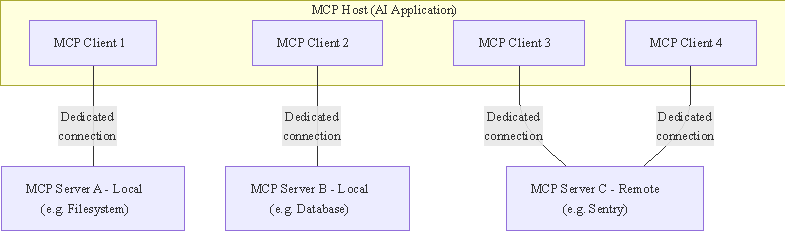
\includegraphics[width=0.95\textwidth]{img/mcp_architecture.pdf}
    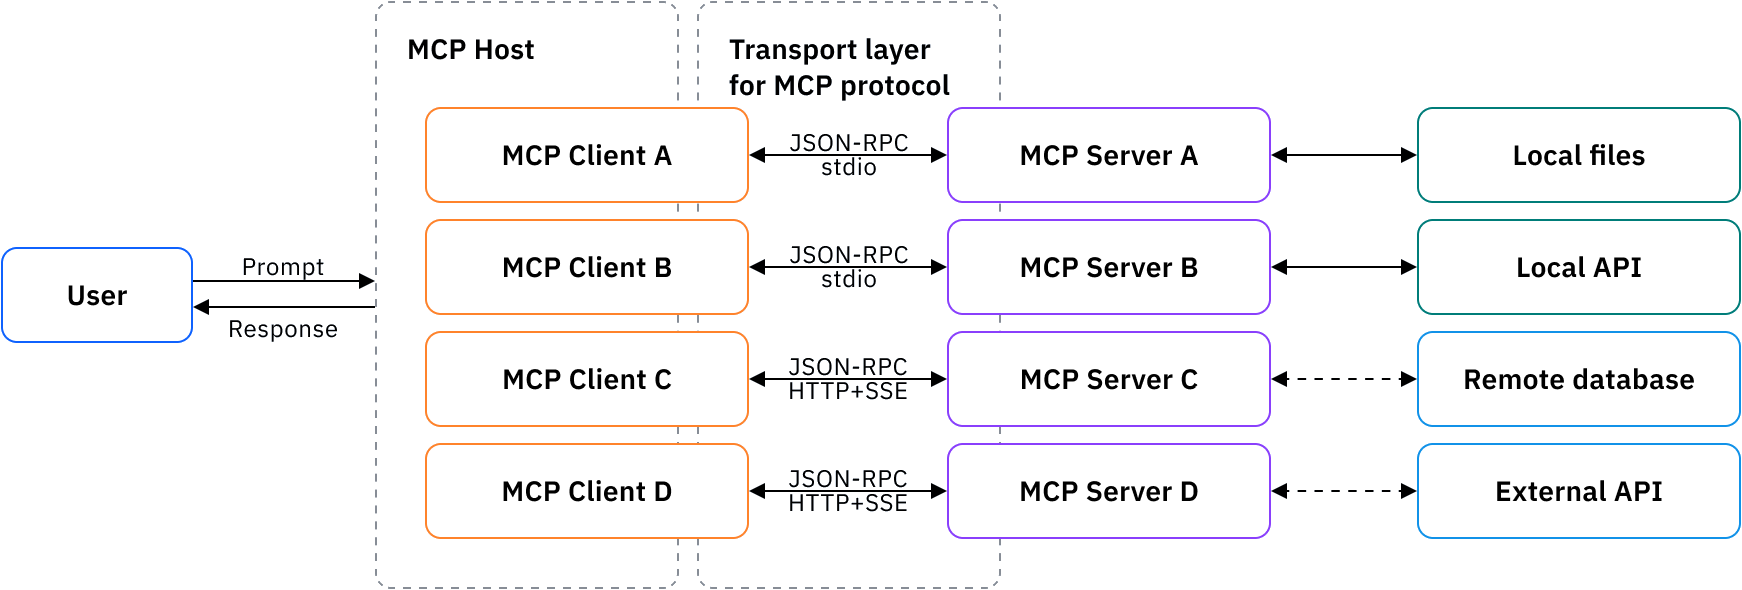
\includegraphics[width=0.95\textwidth]{img/mcp_architecture.png}
    \caption[Architettura del Model Context Protocol]{
        Architettura del Model Context Protocol. Adattata da \cite{gutowska2025mcp}.
        }
    \label{fig:mcp_architecture}
\end{figure}

\section{Reverse engineering assistito} % 2.4

\subsection{LLM nella binary analysis} % 2.4.1

I rapidi progressi nel campo dell'AI hanno portato all'impiego dei LLM anche nel SRE, dove le loro capacità di comprensione e generazione del codice possono essere sfruttate dai reverse engineer per supportare il processo di analisi binaria dei software.

In questo contesto si inseriscono i due lavori descritti di seguito.

\begin{description}
    \item[LLM4Decompile \cite{tan2024llm4decompile}.] Propone una famiglia di LLM open-source, con dimensioni comprese tra $1.3$ e $33$ miliardi di parametri, \textit{fine-tuned} per la decompilazione di codice binario in linguaggio C. L'obiettivo è produrre codice sorgente più leggibile e semanticamente corretto rispetto ai decompilatori tradizionali.
    
    Lo studio introduce due classi di modelli, che seguono approcci complementari, schematizzati nella \Cref{fig:llm_decompile}:

    \begin{itemize}
        \item \textit{LLM4Decompile-End}. Dopo il disassemblaggio del codice binario in istruzioni assembly x86, il modello genera direttamente il corrispondente codice C, ottenendo risultati superiori sia al decompilatore di Ghidra sia a modelli general-purpose come GPT-4o.
        
        \item \textit{LLM4Decompile-Ref}. In questo caso, dopo il disassemblaggio, il codice viene inizialmente decompilato mediante Ghidra; successivamente, il modello utilizza il codice decompilato come punto di partenza per migliorarne leggibilità e correttezza semantica. L'intervento non si limita alla semplice revisione dei nomi e dei tipi delle variabili, ma mira a una rielaborazione più generale del codice, aumentando la potenziale eseguibilità rispetto alla sola decompilazione automatica.
    \end{itemize}

    \begin{figure}[t]
        \centering
        \begin{subfigure}{0.45\textwidth}
            \centering
            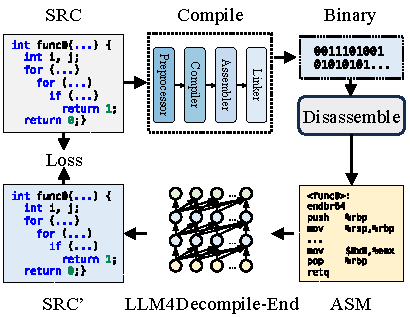
\includegraphics[width=\textwidth]{img/llm_decompile_end.pdf}
            \caption{\hspace{1em} Framework \emph{End2end-Decompile} basato su \emph{LLM4Decompile-End}}
            \label{fig:llm_decompile_end}
        \end{subfigure}
        \hspace{0.05\textwidth}
        \begin{subfigure}{0.45\textwidth}
            \centering
            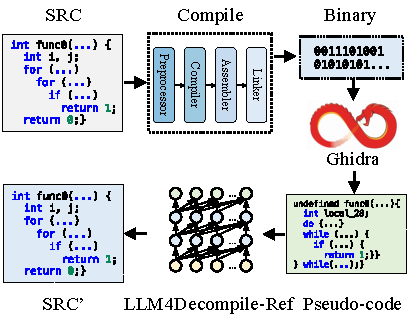
\includegraphics[width=\textwidth]{img/llm_decompile_ref.pdf}
            \caption{\hspace{1em} Framework \emph{Refined-Decompile} basato su \emph{LLM4Decompile-Ref}}
            \label{fig:llm_decompile_ref}
        \end{subfigure}

        \caption[Framework \emph{End2end-Decompile} e \emph{Refined-Decompile}]{
            Framework \emph{End2end-Decompile} e \emph{Refined-Decompile} per la decompilazione del codice binario. Adattata da \cite{tan2024llm4decompile}.
        }
        \label{fig:llm_decompile}
    \end{figure}

    I risultati sperimentali ottenuti con LLM4Decompile mostrano come LLM specializzati possano superare gli strumenti tradizionali di decompilazione, evidenziando il potenziale dei LLM come supporto alle attività di SRE.

    \item[ReCopilot \cite{chen2025recopilot}.] Presenta un LLM specializzato nelle principali attività dell'analisi statica, progettato per operare come un copilota a supporto del reverse engineer durante il processo di analisi.

    ReCopilot adotta un approccio di addestramento articolato in più fasi:

    \begin{itemize}
        \item \textit{Continue Pre-Training} (CPT). Un LLM di base viene ulteriormente pre-addestrato su un ampio corpus di dati relativi al SRE, al fine di acquisire una conoscenza specialistica del dominio e delle relazioni tra codice binario, assembly, codice sorgente e linguaggio naturale.

        \item \textit{Supervised Fine-Tuning} (SFT). Il modello viene quindi specializzato su un insieme di task tipiche dell'analisi statica, imparando a seguire le istruzioni dell'utente e a produrre output in formati strutturati. Tra le attività considerate rientrano la decompilazione, l'analisi delle funzioni e dei relativi nomi, parametri e variabili, a cui si aggiungono task come l'identificazione di algoritmi, la classificazione e la generazione di riassunti relativi a codice e funzioni. Il training include inoltre esempi basati su Chain of Thought, con l'obiettivo di guidare il modello nel processo di ragionamento prima della generazione della risposta.

        \item \textit{Direct Preference Optimization} (DPO). Il modello viene infine ottimizzato rispetto alle preferenze umane, migliorandone la capacità di seguire il formato richiesto e la qualità, la consistenza e la pertinenza delle risposte generate.
    \end{itemize}

    Dal punto di vista sperimentale, ReCopilot supera sia gli strumenti tradizionali di SRE, come IDA Pro e Ghidra, sia gli LLM general-purpose, pur mantenendo dimensioni contenute ($7$ miliardi di parametri rispetto alle dimensioni molto maggiori dei modelli general-purpose). Inoltre, la natura specialistica e strutturata del modello lo rende particolarmente adatto all'integrazione all'interno di sistemi agentici. In questo contesto, ReCopilot può essere impiegato come modulo dedicato all'analisi binaria da parte di un agente di SRE autonomo, al quale può fornire analisi dettagliate a partire da pseudocodice o istruzioni assembly.

\end{description}

\subsection{LLM nella malware analysis}

Dopo le prime applicazioni dei LLM al SRE in contesti generici, il loro impiego è stato progressivamente esteso anche ad ambiti più specifici della cybersecurity, tra cui la malware analysis.

A questo scopo, sono emerse soluzioni specializzate, come quelle presentate di seguito, progettate per sfruttare le capacità dei LLM a supporto dell'analisi dei campioni malevoli e delle attività di SRE.

\begin{description}
    \item[Project IRE \cite{caswell2025projectire}.] Sviluppato da Microsoft, rappresenta uno dei primi esempi industriali di applicazione dei LLM alla malware analysis. Il sistema è progettato per classificare automaticamente un file eseguibile come benigno o maligno disponendo esclusivamente del campione binario, senza fare affidamento su metadati, telemetria o altre informazioni relative alla sua provenienza. L'obiettivo è assistere gli analisti nella gestione dell'elevato numero di file da analizzare, riducendo i tempi e il carico operativo.

    Project IRE adotta un'architettura agentica nella quale un LLM coordina una suite di strumenti specializzati per il SRE. L'architettura consente di combinare diversi livelli di analisi, passando dall'analisi binaria a basso livello alla ricostruzione del control flow, fino all'interpretazione ad alto livello del comportamento del codice. I diversi strumenti, accessibili tramite API, includono sandbox per l'analisi dei campioni, strumenti Microsoft e componenti open source, tra cui decompilatori, strumenti per la ricerca e per il recupero di documentazione.

    Durante l'analisi, il sistema costruisce una \emph{chain of evidence}, ovvero una sequenza di evidenze che documenta il percorso seguito per giungere alla classificazione finale. Questa traccia risulta particolarmente utile durante la revisione da parte degli analisti, poiché consente di verificare le evidenze alla base della classificazione e di individuare i passaggi che possono aver contribuito a un'eventuale decisione errata.

    Le valutazioni preliminari riportano un tasso di classificazione corretta pari a circa il $90\%$ dei campioni analizzati, con una percentuale di falsi positivi prossima al $2\%$. Questi risultati suggeriscono la possibilità di impiegare il sistema in scenari operativi, mantenendo tuttavia la revisione da parte di analisti esperti come componente del processo di analisi.

    \item[MASDroid \cite{wei2026masdroid}.] Propone un framework multi-agente dedicato all'analisi di malware Android. Il sistema combina diversi agenti specializzati con tecniche di analisi comportamentale, producendo una classificazione del malware accompagnata da spiegazioni interpretabili dal reverse engineer.

    L'obiettivo del framework è superare alcune delle principali limitazioni degli approcci esistenti, tra cui la possibilità di elusione delle tecniche di analisi puramente statica, il costo computazionale maggiore dell'analisi dinamica e, soprattutto, la limitata trasparenza dei processi decisionali dei sistemi tradizionali.

    L'architettura di MASDroid, rappresentata anche nella \Cref{fig:masdroid_overview}, può essere suddivisa in tre componenti principali:

    \begin{itemize}
        \item \textit{Static Analysis}: il file APK viene preliminarmente decompilato e analizzato, estraendo un insieme di caratteristiche che viene successivamente fornito ai diversi agenti come base comune per l'analisi.

        \item \textit{Multi-Agent Collaboration}: i diversi agenti operano in parallelo, ciascuno responsabile di una specifica attività di analisi, per cui può utilizzare i tool a disposizione. Gli output prodotti vengono organizzati in un formato strutturato, che combina un \textit{maliciousness score} con una \textit{evidence list}, e vengono successivamente forniti all'agente responsabile della decisione finale.

        \item \textit{Decision Agent}: l'agente di decisione integra le informazioni provenienti dai diversi agenti ed esegue la classificazione finale. Esso genera inoltre un report strutturato contenente lo score finale, i riferimenti alle evidenze e alle attività dei singoli agenti, rendendo il processo decisionale maggiormente interpretabile dal reverse engineer.
    \end{itemize}

    Le valutazioni sperimentali mostrano prestazioni superiori al $97\%$ sia nella rilevazione del malware sia nella classificazione della relativa famiglia. Oltre ai risultati quantitativi, gli autori evidenziano come l'approccio multi-agente migliori l'interpretabilità delle decisioni rispetto ai tradizionali modelli \textit{black-box}, fornendo classificazioni supportate dalle evidenze raccolte durante il processo di analisi.

    \begin{figure}[t]
        \centering
        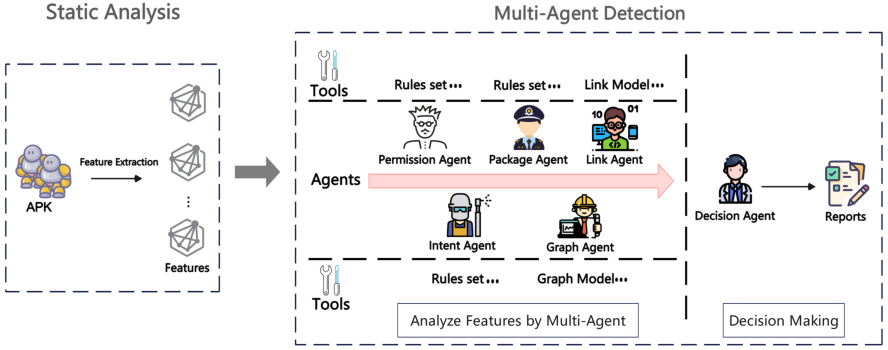
\includegraphics[width=0.95\textwidth]{img/masdroid_overview.pdf}
        \caption[Panoramica dell'architettura di \emph{MASDroid}]{
            Panoramica dell'architettura di \emph{MASDroid}. Adattata da \cite{wei2026masdroid}, \copyright{} 2026 IEEE.
        }
        \label{fig:masdroid_overview}
    \end{figure}

\end{description}

\subsection{Interazione Persona-LLM nel SRE}

La crescente diffusione dei LLM nelle attività di SRE evidenzia come lo stato dell'arte della ricerca si stia progressivamente orientando verso l'integrazione di tali modelli all'interno del flusso di lavoro dei reverse engineer. % la ricerca scientifica e le prospettive future del settore

In questo contesto, tra il 2024 e il 2025, Basque et al. \cite{basque2026srellmstudy} hanno condotto il primo studio sistematico volto a comprendere come gli LLM possano collaborare con i reverse engineer durante le attività di SRE. Lo studio si propone di analizzare le modalità con cui gli LLM vengono integrati nel processo di analisi, il loro impatto sul flusso di lavoro dei reverse engineer e la percezione del loro utilizzo.

% Dopo un sondaggio preliminare che ha permesso di filtrare il pool di candidati.

Per lo svolgimento dello studio, i ricercatori hanno selezionato $48$ partecipanti, equamente suddivisi tra reverse engineer con esperienza limitata ed esperti. I partecipanti sono stati quindi coinvolti in un esperimento controllato, nel quale dovevano analizzare due programmi binari progettati in stile \textit{Capture The Flag} (CTF), contenenti sfide rappresentative di comuni attività di SRE. L'esperimento prevedeva due condizioni, rispettivamente con e senza il supporto di un LLM. Nel secondo caso, ai partecipanti veniva messo a disposizione un plugin per IDA Pro con funzionalità specifiche di analisi basate su LLM, oltre a una \emph{chatbox} per interagire liberamente con un LLM.

% (l'assistenza LLM veniva fornita attraverso un'interfaccia integrata nel flusso di lavoro).

L'osservazione delle attività svolte dai partecipanti ha portato all'individuazione di $18$ risultati sperimentali, successivamente sintetizzati dagli autori in cinque principali conclusioni \cite{basque2026srellmstudy}:

\begin{description}
    \item[Supporto nelle fasi iniziali.] L'uso dei LLM è particolarmente utile nelle fasi iniziali dell'analisi, grazie al fatto che fornisce una visione d'insieme a fronte di un basso costo cognitivo. Questo approccio avvantaggia soprattutto i reverse engineer meno esperti, mentre il beneficio si riduce nel caso di analisi più approfondite.
    \item[Impatto limitato sugli esperti.] L'apporto dei LLM migliora solo marginalmente le competenze degli esperti, i quali preferiscono delegargli le attività di routine, così da riallocare il proprio impegno sulla comprensione di logiche complesse, ridistribuendo così lo sforzo.
    \item[Rischio delle allucinazioni.] Anche delle allucinazioni rare possono compromettere seriamente il flusso di analisi, visto che la formulazione e l'indagine di ipotesi errate prolunga i tempi complessivi di lavoro.
    \item[Recupero degli artefatti vs. compresione semantica.] La comprensione semantica del programma da parte del reverse engineer dipende fortemente dal recupero degli artefatti. Nonostante i LLM aiutino a recuperare tipi, nomi di funzioni e variabili, questo non si traduce automaticamente in una comprensione profonda del funzionamento del codice.
    \item[Limiti nella delegazione delle attività.] Ai LLM possono essere demandate solo le attività più semplici, come ad esempio la descrizione e la caratterizzazione di funzioni \textit{single-purpose} e di algoritmi standard. Nel caso di funzioni complesse, con più ruoli o dotate di logiche intricate è necessaria un'analisi umana iterativa, eventualmente supportata dai LLM.
\end{description}

% Our study takes the first in-depth empirical dive into how LLMs impact SRE and demonstrates that they augment analysts rather than replace them. The benefits are clear: LLMs support SRE practitioners in many tasks and can even close the gap in some aspects between experts and novices. However, our study shows that many areas of LLM integration still require research and development to be helpful for the most challenging SRE tasks. We present our findings, hopeful that the SRE community will utilize our work to make LLMs an even more helpful tool for security. All in all, LLMs are neither oracles nor impostors, but mirrors held to human insight: their reflections sharpen only in the steady gaze of critical thought and domain expertise.

% Vantaggi uso LLM: spiegare comportamento di codice decompilato e funzionamento algoritmi, aumento leggibilità, identificazione (renaming), velocizzazione del processo di SRE con la creazione di script di supporto. Svantaggi uso LLM: risposte incorrette o misleading, riducendo la fiducia o causando perdita di tempo, spiegazioni superficiali, con diminuzione generale dell'efficacia al complicarsi e all'allungarsi della task.

Lo studio evidenzia dunque che, in assenza di un avanzamento tecnologico nell'ambito della GenAI, di un miglioramento delle conoscenze specifiche dei LLM e, soprattutto, di un'evoluzione delle modalità di interazione, questi modelli rimarranno per la maggior parte degli strumenti di supporto per principianti, piuttosto che veri collaboratori alla pari per gli esperti di SRE \cite{basque2026srellmstudy}.

% A Survey on Agentic Security: Applications, Threats and Defenses (https://arxiv.org/pdf/2510.06445): descrive l'utilizzo degli agenti LLM-based nella cybersecurity.

Tuttavia, è fondamentale sottolineare che tale conclusione è stata formulata considerando una modalità di interazione basata su assistenti conversazionali e sullo stato dell'arte della GenAI precedente alle più recenti evoluzioni. La diffusione, tra il 2025 e il 2026, dei sistemi agentici basati su LLM ha contribuito ad affermare un paradigma di interazione differente, nel quale il modello può pianificare autonomamente le attività da svolgere, utilizzare strumenti e modificare le proprie azioni sulla base dei risultati ottenuti. Questo approccio può quindi modificare il ruolo dei LLM nella SRE, spostandolo da una funzione prevalentemente assistiva a forme di collaborazione caratterizzate da una maggiore autonomia.

Proprio in questa direzione si sviluppa il lavoro di Radey et al. \cite{radey2026challenges}, che analizza le capacità tecniche dei sistemi agentici applicati alla SRE e propone una classificazione basata sulle modalità di analisi adottate. Gli autori distinguono tra \emph{static analysis agents}, che si concentrano prevalentemente sull'analisi statica del codice decompilato, e \emph{hybrid agents}, che combinano attività di analisi statica e dinamica. Un'ulteriore distinzione riguarda il grado di autonomia con cui i sistemi operano. Nei sistemi \emph{human-in-the-loop}, il reverse engineer mantiene un ruolo attivo nel processo, verificando le azioni dell'agente e garantendo che l'analisi venga svolta in sicurezza. Nei sistemi autonomi, invece, gli agenti possono condurre autonomamente il processo di analisi, coordinandosi e comunicando tra loro senza un intervento umano diretto.

% L'analisi dinamica non viene considerata da sola, ma viene unita con quella statica. Questo perché l'analisi dinamica rimane più difficile da scalare rispetto a quella statica e i componenti interattivi e adattivi dell'analisi dinamica la rendono più difficile da eseguire indipendentemente da un umano per un LLM.

Nonostante le potenzialità del paradigma agentico, lo studio evidenzia diverse limitazioni dei sistemi attuali negli scenari realistici e complessi di SRE \cite{radey2026challenges}. Le capacità di analisi possono essere compromesse dall'offuscamento del codice, complicandone la ricostruzione semantica, in modo analogo a quanto già avviene nell'analisi condotta da un reverse engineer umano. A ciò si aggiungono i vincoli di contesto dei LLM, la difficoltà di controllare il processo di ragionamento dell'agente e le problematiche legate all'ambiente di esecuzione, tra cui la gestione sicura dei comandi impartiti dall'agente. Infine, è necessario considerare il compromesso tra autonomia e supervisione: un ragionamento non supervisionato può portare l'agente a seguire direzioni poco produttive, riducendo l'efficacia dell'analisi, mentre il coinvolgimento umano consente di avere maggiore controllo, a scapito dell'autonomia del sistema.

% Vincoli di contesto che possono limitare la quantità di informazioni considerate durante l'analisi.

Il paradigma agentico rappresenta dunque una naturale evoluzione dell'impiego dei LLM nella SRE, ma è ancora in una fase iniziale e in rapido sviluppo, come testimonia la crescente attenzione della ricerca verso questi sistemi. La loro efficacia deve ancora essere verificata in maniera estesa in scenari realistici, anche attraverso benchmark capaci di catturare adeguatamente le caratteristiche delle attività tipiche di reverse engineering. Le sfide future non riguarderanno quindi soltanto il miglioramento dei LLM, ma anche la progettazione di agenti AI robusti in grado di sfruttarne pienamente il potenziale, integrandoli efficacemente con gli strumenti e gli ambienti di analisi, così da garantire autonomia e affidabilità al processo di reverse engineering.

% Se gli agenti verranno impiegati per automatizzare una parte sempre maggiore della SRE, gli avversari potranno infatti adattare i propri binari non soltanto per ostacolare il reverse engineer umano, ma anche per sfruttare le specifiche limitazioni dei sistemi agentici.